\section{실험 설정}

\begin{figure*}[!t]
\centering
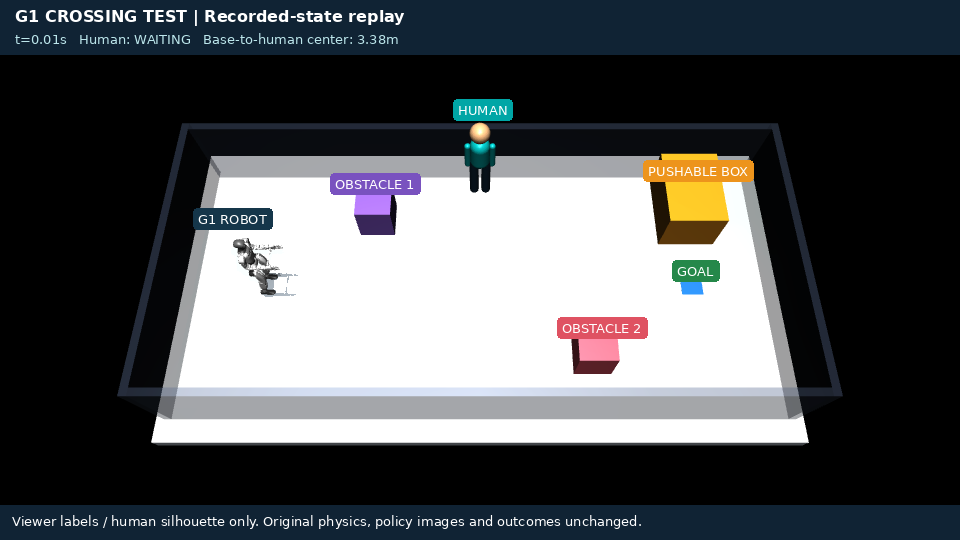
\includegraphics[width=0.42\textwidth,valign=c]{figures/humanoid_scene.png}\hfill
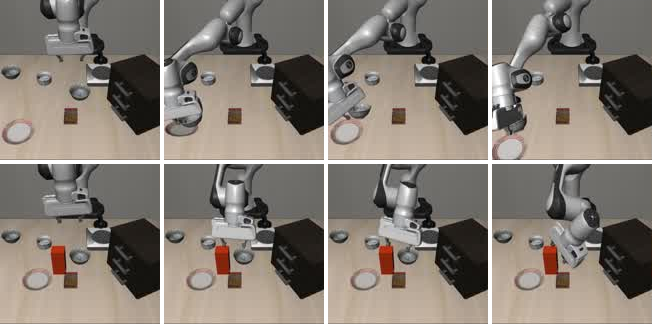
\includegraphics[width=0.56\textwidth,valign=c,trim=0 164 0 0,clip]{figures/arm_failure_frames.png}
\caption{실험 환경. (좌) G1 휴머노이드 횡단 장면: 장애물 2개, 밀 수 있는 상자, 목표, 이동하는 사람.
(우) LIBERO 로봇팔 장면: 테이블 중앙의 검은 그릇을 접시 위로 옮기는 과제.}\label{fig:env}
\end{figure*}

\begin{table*}[!t]
\centering\small
\caption{두 실험의 주요 조건 (세부 설정은 부록 A)}\label{tab:setup}
\begin{tabularx}{\textwidth}{@{}p{28mm}YY@{}}
\toprule
항목 & 실험 1: 로봇팔 pick-and-place & 실험 2: 휴머노이드 이동 \\
\midrule
로봇·정책 & LIBERO~\cite{libero}의 Franka Panda~\cite{panda} + GR00T~N1.7 (VLA)~\cite{groot,grootrepo} & Unitree G1~\cite{g1} + LLM Agent·경로 계획·GR00T 보행 제어~\cite{wbc} \\
작업 & 검은 그릇을 집어 접시에 놓기 & 상자·장애물·횡단하는 사람이 있는 통로에서 목표 도달 \\
환경 축 & 10 (그릇·접시 XY, 장애물 위치·크기·높이·회전) & 21 (물성, 통로 폭, 장애물 2개, 상자, 사람) \\
반복·예산 & 난수 시드 3개 $\times$ 방법별 4회 = 방법별 12회 & 난수 시드 1개, 방법별 유효 5회 \\
초기 장면 & 시드별 처음 2회는 양 방법 공통 무작위 장면 & 양 방법 공통 기준 장면 1회 \\
탐색 LLM & GPT-6 Luna Pro~\cite{luna}, 제안 6회 & GPT-6 Luna Pro~\cite{luna}, 제안 4회 \\
\bottomrule
\end{tabularx}
\end{table*}

그림~\ref{fig:env}는 두 실험의 환경이고, 표~\ref{tab:setup}은 주요 조건이다. 두 실험 모두 AFS와 Random은 같은 로봇, 작업, 성공 판정, 환경 변경 범위, 시도 예산을 사용한다.
AFS는 같은 시드 안의 자기 실행 이력만 참고하며, 다른 방법이나 과거 실험의 결과를 가져오지 않는다.
